
\chapter{Background}\label{chap:background}
\section{Markov Decision Process}

\cite{bellamn1957mdp} described a framework for solving stochastic control problems. A classic example of this is playing blackjack. There is often no certain outcome to playing a given hand. However, actions exist for which the expected probability of a player winning is higher. The Markov Decision Process (MDP) formalism allows one to tackle such problems systematically, with mathematically tractable convergence bounds to optimal solutions in some cases.

The MDP describes these processes as an agent acting in an environment that is, in general, partially observable.

This is described by a tuple $(\mathcal{S}, \mathcal{A}, \mathcal{R}, P, \gamma)$. $\mathcal{S}$ is the state space, the state of the world that the agent knows about, and $\mathcal{A}$ is the action space, the possible actions it may take. For a given state and action, the reward provided is real-valued and may be stochastic, $\mathcal{R}: \mathcal{S} \times \mathcal{A} \rightarrow \mathbb{R}$. $P$ are the transition probabilities between states $P: \mathcal{S} \times \mathcal{A} \times \mathcal{S} \rightarrow [0, 1]$, this defines the dynamics of the process. $\gamma $ determines the reward discount, how myopic the MDP is.

The agent aims to maximize its expected discounted cumulative reward, the return,
\begin{equation}
	\mathbb{E} [ G_t = \sum_t^T \gamma^t R_t ] .
\end{equation}
The problem may be that of an episodic setting with a clear termination, a chess player winning, for example. Alternatively, it may be in a continuous setting with no clear termination, like managing stocks. To make decisions, an agent follows a policy. The policy, $\pi(a|s), \pi: \mathcal{S} \times \mathcal{A} \rightarrow [0, 1]$ maps states' actions to probabilities of taking action $a$. In the deterministic case it is just a map from state to action space.


A family of algorithms known as dynamic programming exists that, given finite states and actions, can find exact solutions to these problems, under reasonable constraints. However, these algorithms are often intractable for large state and action spaces. This is due to their algorithmic complexity being bounded by $\mathcal{O}(|\mathcal{S}||\mathcal{A}|)$.

Solutions to MDPs can be expressed in terms of the value function, $V(s) = \mathbb{E} [ G_t | s_t = s]$, which is the expected return from a given state.

The optimal value function, $V^*(s)$, is the maximum value function over all possible policies. The optimal deterministic policy, $\pi^*(s)$, is the policy that maximizes the value function for all states. The optimal value function and policy satisfy the Bellman optimality equations\cite{bellamn1957mdp}:
\begin{equation}
	V^*(s) = \max_a \mathbb{E} [ R_{t+1} + \gamma V^*(s_{t+1}) | s_t = s, a_t = a].
\end{equation}

The value function is very closely linked to the action-value function $Q(s, a) = \mathbb{E} [G_t | s_t=s, a_t,=a]$ which is the expected return from taking action $a$ in state $s$ and then following the current policy. There also exists a bellman optimality equation for the action-value function:
\begin{equation}
	Q^*(s,a) = \mathbb{E} [ R_{t+1} + \gamma \max_{a'} Q^*(s_{t+1}, a') | s_t = s, a_t = a].
\end{equation}

Reinforcement learning is a common alternative to dynamic programming, which provides a principled approach to learning approximate solutions. It describes a family of techniques that learn from previous experience to improve at solving MDPs.

\section{Reinforcement Learning}
Reinforcement Learning (RL) encompasses the techniques used to solve MDPs where experience is required to solve the MDP. Especially in Deep RL, gradient based function approximations are used to parametrize either policies or value functions. Despite the approximate nature of their solutions, RL agents have achieved superhuman performance in Chess, Go, Star-Craft and have recently found diamonds in Minecraft~\cite{silver2016mastering,silver2017mastering,hafner2023mastering}. Many of these successes with current RL approaches highlight the challenges current algorithms face due to their hunger for data. This poor sample efficiency, is permissible in game environments as they are cheap to sample from. Even in the video game setting, these agents took millions of dollars, and many hours of compute. In real world tasks the costs of gaining samples is more expensive and presents an even larger challenge.

This sample hunger, combined with the challenge of to transfer knowledge between tasks~\cite{kirkpatrick2017overcoming}, highlights that there is a significant advantage to encoding prior knowledge into RL algorithms. The knowledge of symmetries enables agents to attempt simplified problems and draws abstract connections between different tasks. This thesis focuses on the encoding of symmetries into RL algorithms. Before introducing symmetry rigorously, this section will describe the most common approaches to solving complex RL problems.

\section{Deep Reinforcement Learning Approaches}
The underlying optimization problem in reinforcement learning is finding a policy which produces the maximum expected return. However, not all RL algorithms directly maximize return. The techniques used to train agents are broadly separated into two categories: Model-free and model-based algorithms.

Model-free algorithms choose to forgo learning the dynamics of a process and instead model the value function or policy directly.

In contrast, model-based algorithms learn the problem's dynamics and simulate the results of agent's behaviour in an environment to learn. This section will describe the most common approaches to solving RL problems.
Typically, learning algorithms face a few persistent problems in Deep RL that make solving problems difficult. A non-exhaustive list is:
\begin{itemize}
	\item \textbf{Sample Efficiency} The algorithms require a large amount of data to learn. This is because training large neural networks are sample inefficient, taking tens hours to learn tasks such as playing Atari~\cite{hessel2018rainbow}, which humans can do in minutes. As mentioned before, breakthroughs in RL are often made in games, where data can be simulated and collected cheaply\cite{dulac2019challenges}
	\item \textbf{Training Robustness} The algorithms can often struggle to converge depending on the initialization of the environment and the agent, and special random seeds are required to see good performance\cite{henderson2018deep}.
	\item \textbf{Reward Sparsity} Reward functions are often sparse, and coming across states that provide rewards, such as finding diamonds in Minecraft, is a difficult problem when initial exploration is random~\cite{hafner2023mastering}.
	\item \textbf{Deadly Triad} many algorithms use their own predictions to update their current behaviour, a process known as bootstrapping. This in conjunction with off-policy learning can lead to Q-value divergence~\cite{van2018deep}, and an inability to learn.
	\item \textbf{Catastrophic Forgetting} like in the context of supervised learning, deep networks have the problem that when trained on sequential tasks they loose performance on previous tasks in the sequence~\cite{kirkpatrick2017overcoming}. These problems can be somewhat overcome by storing experience in the MDP and always using this to update the agent.

\end{itemize}



\subsection{Model Free Algorithms}
Model free algorithms attempt to train an agent to maximize returns from agent experience. The two key paradigms either approximating a value function are, Q-learning. Or the agent learns the best action to take in given states these are policy gradient methods.

When combining standard dynamic programming algorithms such as Q-learning with function approximation, or direct policy learning, the challenge is finding a way to learn the form of the parametric function approximator, which is often a neural network. As such, there is a common approach between multiple algorithms, where you form a supervised learning problem, finding a function that minimizes a loss. In the RL setting, the data is gained from the MDP. The fundamental difference between Q-Learning and Policy Gradient approaches is that Q-learning uses an epsilon greedy policy to collect experience. Whereas, Actor Critics learn and gain experience with the same policy. However, the training loop is much the same;

\begin{algorithm}
	\caption{Intuition For Model Free RL Training Loop}
	\begin{algorithmic}
		\State Initialize $\theta$ randomly.
		\Comment{Network Parameters}
		\State Initialize $t=0$
		\Comment{Buffer Timestep}
		\State Initialize $T=0$
		\Comment{Total Timestep}
		\State Initialize replay buffer $\mathcal{D} \leftarrow \emptyset$
		\State Sample state $s$
		\While $\text{ }T < T_{max}$
		\State Take action $a$ according to policy $\pi(a|s)$
		\State Observe reward $r$ and next state $s'$
		\State Store transition $(s, a, r)$ in replay buffer $\mathcal{D}$
		\If{$t \mod T_{experience} = 0$}
		\Comment{ Update Loop}
		\State Perform gradient-based learning update
		\State $t \leftarrow 0$
		\State $\mathcal{D} \leftarrow \emptyset$
		\EndIf

		\EndWhile

	\end{algorithmic}
\end{algorithm}
In most cases, some operations need to be performed on the replay buffer, and the buffer will store more data than just sequential $(s, a,r)_t$ tuples. Some might argue that replay buffers are not required in certain algorithms, but this is just the case of a single transition long replay buffer. Often subsequent actions are required to calculate the loss. This can be done during the update loop. Finally, rather than interacting with one environment, training can be done in parallel in multiple environments. The process is much the same; states, rewards and actions become vectors for this. Environment vectorization has improved training stability and robustness~\cite{minh2016asynchronous}.

\subsubsection{Deep Q-Learning}\label{sec:Q-learning}
Q-Learning forgoes optimizing the true objective, the policy, to learn the optimal value function. This allows one to find an optimal policy, as there is always a deterministic greedy policy, $\pi^*(s) = \arg \max_{b} Q^*(S, b)$, with a stationary point at the optimal value function.

Such ideas are the foundations of Dynamic Programming, which exploits this idea in algorithms such as Value Iteration\cite{bellamn1957mdp} and Policy Iteration\cite{howard1960dynamic}.

When extended to function approximation the convergence guarantee of the original dynamic programming Q-learning algorithm is absent in Deep-Q-Learning. While an exact solution may not be found due to computational constraints, excellent solutions can be found in practice using this method~\cite{mnih2013playing}. Traditional Q-learning updates the value of the current state-action pair, $Q(s, a)$, using the Bellman optimality equation for the action-value function,
\begin{equation}
	Q_{t+1}(s, a) = Q_t(s,a) + \alpha \left[ r(s, a) + \gamma \max_{a'} Q_t(S_{t+1}, a') \right].
\end{equation}
Where $\alpha$ is the step size, all other symbols take their normal values. The important point is that this converges to the optimal value function given infinite state action space visitation. In the setting of Deep Q-Learning, we lose the guarantees of convergence in exchange for the ability to attack problems that have large on continuous state-action spaces. An important point to note about Q-Learning is that the agent uses its own predictions to learn. This is known as bootstrapping and can cause problems, famously the deadly triad~\cite{van2018deep,sutton2018reinforcement}.

The Bellman optimality equation can be used to construct a loss function to train a parametric function approximation, a deep learning model, through gradient methods, If this method were employed in an on-policy fashion with a deterministic greedy optimal policy, there would be no exploration. As such, the agent would not gain new experience, so an alternative exploration policy is used, which alternates between greedy and random actions. The results of its trajectory or trajectories, depending on whether it is an episodic setting, are stored in a replay buffer,
\begin{equation}
	\mathcal{D} = \{S_0, A_0, R_1, S_1, A_1, \ldots \}
\end{equation}
This can be sampled when training the network. The loss function to optimize is derived from the Bellman equation and is the squared temporal difference error\cite{sutton2018reinforcement},
\begin{equation}
	L_{w}(\mathcal{D}) = \mathbb{E}_{(s,a,r,s') \sim \mathcal{D}}\left[\left(Q_w(s,a) -(r + \gamma(1-\mathbb{I}(s'= S_{T}))\max_{a'}Q_{w'}(s', a')\right)^2\right].
\end{equation}
Here, it is essential to note that $Q_w'$ can be the original network if $w = w'$. However, there are some problems associated with this. The gradient with respect to the loss must now become a semi-gradient, to allow the bootstrapping off one's own predictions, where the $Q_w'$ term must be considered a constant with respect to $w$. The indicator, $\mathbb{I}(s' = S_T)$,  is one if $s'$ is a terminal state.

Alternatively, the semi-gradient can be avoided with Double-Q-Learning. Double-Q-Learning uses target networks~\cite{van2016deep}. This makes two copies of the primary, $Q_w$, network and performs gradient updates on one, $Q_w$, with the secondary network, $Q_{w'}$, parameters being moved towards $w$ after some further number of updates so that its parameters lag that of $w$. This can be done with weighted averages or just a direct update.

Some problems arise in continuous state spaces, where the $\max$ operation may involve an optimization loop. This is not ideal. Algorithms such as Deep Deterministic Policy Gradient (DDPG)\cite{lillicrap2015continuous} use another network to parametrize an optimal policy instead of the max operation. DDPG is an example of an Actor-Critic algorithm that straddles the divide between Q-Learning and policy based methods.


\subsubsection{Policy Based Methods}
Policy based methods aim to learn an optimal policy directly. Policy based methods strive to optimize the expected cumulative return for an agent by performing gradient descent on the obtained rewards. The return for a given action, is not known beforehand and must be estimated. Reducing the variance of the estimator is a key challenge. There are multiple tricks used in deriving the gradient estimator to reduce variance as well as algorithmic improvements such as Soft Actor-Critic (SAC)~\cite{haarnoja2018soft}, Proximal Policy Optimization (PPO)\cite{schulman2017proximal}.

In the episodic setting, where it is possible to obtain complete trajectories and optimize for episodic returns, policy gradient functions can directly optimize the expected cumulative reward,
\begin{equation}
	J_G(\theta) = \mathbb{E}_{s_0 \sim d_0}\left[v_{\pi_{\theta}}(S_0)\right].
\end{equation}
However, in infinite time horizon tasks, there is no termination and optimizing for the expected reward of the next action may be a more prudent objective,
\begin{equation}
	J_R(\theta)
	= \mathbb{E}_{\pi_{\theta}}\left[R_{t+1}\right].
\end{equation}
Many common algorithms for episodic tasks can be extended for infinite time horizon problems. In the rest of the report, the episodic setting is only considered.

The general policy gradient is of the form,
\begin{equation}
	\nabla J_G(\theta)  = \mathbb{E}_{\tau \sim \pi_\theta} \left[\sum_{t=0} ^ T \mathcal{R}_t \nabla_\theta \log(\pi_\theta(A_t|S_t))\right].
\end{equation}
Where $\mathcal{R}_t$ is a return estimator a time $t$, if the return estimator is the discounted sum of rewards, this is the REINFORCE algorithm~\cite{williams1992simple}.
The most used modern policy gradient algorithms take this form: a return estimator, which is either sampled or bootstrapped with a possible constant baseline offset. This leads to Actor-Critic methods, where the actor is the policy network, and the critic is a value function estimation network.

\subsubsection{Actor Critic Methods}\label{sec:Actor-Critic}
Actor critics, are a hybrid approach between policy gradient methods and value based methods. In Deep RL  they consist of a pair of function approximation networks, one the actor to approximate the optimal policy, the critic to approximate the optimal value function. Because the gradient of a constant is zero, having a baseline that is independent of the policy does not affect the expectation of the policy gradient estimator, but if picked wisely, it may reduce the variance,
\begin{equation}
	\nabla J_G(\theta)  = \mathbb{E}_{\tau \sim \pi_\theta} \left[\sum_{t=0} ^ T (\mathcal{R}_t - b) \nabla_\theta \log(\pi_\theta(A_t|S_t))\right].
\end{equation}
As the variance of the updates depends on the magnitude of the $(\mathcal{R}_t - b)$ term, a function is learned to estimate the value of the state, $V_\phi(S_t)$, and the baseline is set to the value of the state, $b = V_\phi(S_t)$. The critic trained to minimize the mean squared error between the estimated value and the actual return. This produces an unbiased update of lower variance, which has better training behaviour\cite{sutton2018reinforcement}.

\subsubsection{Generalized Advantage Estimation}
Generalized advantage estimation\cite{schulman2015high}, learns the $\lambda$-return, a weighted sum of the n-step discounted returns, in contrast to learning the discounted return of previous methods. The $\lambda$-return is defined as,
\begin{equation}
	R_t^\lambda = (1-\lambda) \sum_{n=1}^\infty \lambda^{n-1} R_{t:t+n}^V.
\end{equation}
Where $R_{t:t+n}^V$ is the n-step discounted return and lambda is a hyperparameter that controls the trade-off between bias and variance on the return estimator as it gradually uses its own estimates for states values, when $\lambda = 0$, it is an unbiased return estimate. The n-step discounted return is defined as,
\begin{equation}
	R_{t:t+n}^V = \sum_{k=0}^{n-1} \gamma^k r_{t+k} + \gamma^n V_\phi(S_{t+n}).
\end{equation}
The lambda return provides a biased but lower variance return estimator, which can benefit training and is the backbone of many modern policy gradient algorithms. Typically, the lambda return is calculated recursively backwards in episodic settings,
\begin{equation}
	R_t^\lambda = r_t + \gamma (1-\lambda) V_\phi(S_{t+1}) + \lambda R_{t+1}^\lambda.
\end{equation}
And then the advantage is the difference between the value function and the lambda return,
\begin{equation}
	A_t^\lambda = R_t^\lambda - V_\phi(S_t).
\end{equation}
Having the generalized advantage as the optimization target provides control over the variance of the gradient estimator. The generalized advantage estimator is defined as,
\begin{equation}
	\nabla J_G(\theta)  = \mathbb{E}_{\tau \sim \pi_\theta} \left[\sum_{t=0} ^ T A_t^\lambda \nabla_\theta \log(\pi_\theta(A_t|S_t))\right].
\end{equation}
In this situation, the critic network learns to minimize the advantage. Advantage estimation is often used with regularization methods that stop the current policy from moving too far between training updates. These regularization methods penalize the KL divergence between the current and previous policies. This is the case for Trust Region Policy Optimization (TRPO)~\cite{shculman2015trust} and the computationally efficient and simple PPO\cite{schulman2017proximal}.

\subsubsection{PPO}\label{sec:PPO}
Proximal policy optimization (PPO) follows the same lines as TRPO, as it is a regularized form of gradient-based policy optimization with a critic that learns a value function as a bias reduction method. The PPO paper introduces two forms: a hard threshold method PPO-Clip, and a soft regularization method PPO-Penalty. The clip optimization target, that removes the need for explicitly calculating a KL-divergence for a single interaction is,
\begin{equation}
	L(s, a, \theta_k, \theta) = \min \left( \frac{\pi_\theta(a|s)}{\pi_{\theta_k}(a|s)} A^{\pi_{\theta_k}}(s,a), g\left(\epsilon, \frac{\pi_\theta(a|s)}{\pi_{\theta_k}(a|s)} \right)A^{\pi_{\theta_k}}(s, a) \right).
\end{equation}
Where the update rule is defined by the gradient descent algorithm, and $\theta_k$ is the previous value of $\theta$. The advantage of a policy $\pi$ is given by a truncated $\lambda$-return,
\begin{equation}
	A^{\pi}(s, a) = V^\pi _\phi(s) - R_t(s, a).
\end{equation}
Where the $V^\pi _ \phi(s)$ is the critic, typically a neural network. $R_t(s, a)$ is the sampled return for the state action pair. As the algorithm is on-policy, there is an importance-sampling correction to the advantage. To stop wide variance in the policy, like TRPO, the magnitude of the update is capped with the $g$ function,
\begin{equation}
	g(\epsilon, A) = (1 + \text{sign}(A)\epsilon)A.
\end{equation}
The $\epsilon$ hyperparameter must be set. This loss function ensures that there are no overly large policy updates.

\subsection{Model Based Algorithms}
Model-based reinforcement learning is the process of the agent learning the dynamics of a system and then performing ``planning" to decide how best to act next. In concrete terms, this corresponds to an agent learning the transition dynamics of the MDP, thus learning both the subsequent state of a state action pair, $P(s'| s, a)$ and the expected reward from a state action pair $r(s, a)$. From the learned model agent ``plans" by simulating the environment and acting in the simulated environment. Then the agent learns a policy with the simulated data. Common algorithms like Dyna-Q~\cite{sutton2018reinforcement}, use Q-learning over a combination of real and simulated data to learn a policy.

Model-based algorithms have the potential to provide much better sample efficiency than model-free algorithms, as they can learn from simulated data. However, this in itself can be difficult to learn. In cases where the state-action space is infinite the model must generalize to states-actions that have not been seen before. However, the Dreamer models have shown substantial success in tackling difficult problems\cite{hafner2023mastering, hafner2020mastering}.

\section{Dyna} \label{sec:Dyna}
Dyna style algorithms\cite{sutton2018reinforcement, sutton2012dyna} augment model free algorithms, while using the same experience based updates, such as Q-learning~\ref{sec:Q-learning} or PPO~\ref{sec:PPO}, they train, $T(S_{t+1}|S_t, A_t)$ a transition model. This can improve the sample efficiency of an agent. The basic Dyna formulation is outlined in pseudocode below.
\begin{algorithm}\label{algo:Dyna}
	\caption{Dyna}
	\begin{algorithmic}
		\State Initialise $\theta, \phi, \psi,$ randomly
		\For {Num Epochs}
		\For {Num Dyna Iterations}
		\For {Num Acting Updates}
		\State Sample transition tuples from policy $\pi_\theta \sim (s, a, s')$ on $\mathcal{M}$
		\State Construct replay buffer from transitions $\mathcal{D} = \{(s, a, s', r)_i\}_1^N$

		\State $\theta' \leftarrow$ Minimize $L_{a}(\theta, \mathcal{D})$
		\State $\phi' \leftarrow $Minimize $L_{mb}(\phi , \mathcal{D})$
		\State $\psi' \leftarrow $Minimize $L_{rw}(\psi , \mathcal{D})$
		\EndFor
		\State $\theta \leftarrow \theta'$
		\State $\phi \leftarrow \phi'$
		\For{Num Planning Updates}
		\State Sample transition tuples from policy $\pi_\theta \sim (s, a, s')$ on $T_\phi$
		\State Construct replay buffer from planned transitions $\mathcal{D}_{p} = \{(s, a, s', r)_i\}_1^N$
		\State $\theta' \leftarrow$ Minimize $L_{a}(\theta, \mathcal{D}_p)$
		\EndFor
		\State $\theta \leftarrow \theta'$
		\State $\emptyset \leftarrow \mathcal{D}$
		\State $\emptyset \leftarrow \mathcal{D}_p$
		\EndFor
	\end{algorithmic}
\end{algorithm}
Here; $L_{a}$, $L_{mb}$, and $L_{rw}$ are the agent, transition model and reward model losses, respectively. The minimization is typically through stochastic gradient descent.

Dyna provides a conceptually simple model based augmentation on conventional model free algorithms. By simulating transitions using previous experience, higher sample efficiency may be gained at the cost of a more complex training regime.

Next, the mathematical abstractions to deal with symmetries are introduced such that the methods to form inductive biases in RL agents can be understood.
\section{Groups, Symmetries, Homomorphisms}

\subsection{Groups}
Groups are an abstract mathematical idea on a set with a binary operation, $(\text{\_}\cdot \text{\_})$. To form a group, the members of a set must satisfy the following:
\begin{itemize}
	\item[1] Closure: applying the group's operation maps all elements back onto another element.
	\item[2] Possession of an identity element: there must be an element of the set such that it and any element is mapped onto itself.
	\item[3] Possession of inverse elements: every element in the group has an inverse element.
	\item [4] Associativity: $(a \cdot b) \cdot c = a \cdot (b \cdot c) \text{  }\forall a, b, c$
\end{itemize}
The key point is that specific symmetries form groups of all the transformations that leave the object/space invariant. An example of a group table can be found below for the cyclic group $C_2$ in section~\ref{sec:cartpole}.

\subsection{Representation and Actions}
Members of groups like rotation operations or flip operations maintain their properties no matter what space you are in. For example flipping an image or a function the group is still the same, in that if you perform two flips you get the same image/function. As such, the group is a very general and abstract concept. When dealing with groups, in a concrete setting then the group is a set of matrices or functionals that operate on a space or a function, these are in general described as group actions, for our purposes only the left action is needed. The left and right actions refer to the side of the operand the operator is applied. The group action is defined as,
\begin{equation}
	\ell_g: \mathcal{X} \times G \rightarrow \mathcal{X}, \forall g \in G, \forall x \in \mathcal{X}.
\end{equation}
Where $\mathcal{X}$ is an arbitrary set and the left action obeys the following properties:
\begin{itemize}
	\item[1] $\ell_{g_1}(\ell_{g_2}(x)) = \ell_{g_1 \cdot g_2}(x)$.
	\item[2] $\ell_e(x) = x$.
\end{itemize}
Additionally, because of the definition of a group action, the application of a group action to a function is equal to the function applied to the inverse of the group action applied to the function's domain, i.e.
\begin{equation}
	\ell_g(f(x)) = f(\ell_{g^{-1}}(x)).
\end{equation}

The inverse group action is commonly written as $\ell_{g^{-1}}(x) = g^{-1}x$, when acting on the domain of a function.

In the special case of vector spaces the group actions are invertible matrices and are called a representation;
\begin{equation}
	\pi_g^\mathcal{V}: G \rightarrow GL(\mathcal{V}), \forall g \in G.
\end{equation}
Where $\mathcal{V} \in \mathbb{R}^n$ is a vector space, and the group representation $\pi_g^\mathcal{V}$ is an invertible matrix. These representations also follow the properties of the group, i.e. they are invertible, and the identity element is mapped to the identity matrix.
\subsection{Invariances}
Invariances are properties maintained under a transformation of the input space, e.g.\ mirror symmetry, where the distance to a point on the mirror line is the same from the left and the right if the object is symmetric. If you have a function $f: \mathcal{X} \rightarrow \mathcal{Y}$ that is invariant to a transformation $\ell_g(x): \mathcal{X} \times G \rightarrow \mathcal{X}$, this is expressed as:
\begin{equation}
	f(x) = f(\ell_g(x)),   \forall g \in G, \forall x \in \mathcal{X}.
\end{equation}
For the transformation to be a group, there must also include the identity element s.t $\ell_h(x) = x,  h \in G, \forall x\in \mathcal{X}$. From this definition one sees that symmetries themselves are invariances with respect to the action of a group. For example, suppose an object has 3-fold rotation symmetry around an axis. In that case, an abstract group with operations between its elements mirrors that of rotations around the axis by $120^o, 240^o$ and $0^o$. It is straightforward to check that these operations form a group. Rotations by $360^o$ left or right are the identity element. The group is closed; no matter how many rotations are performed, the object with the symmetry is still the same. The inverse of the rotation by $120^o$ is the rotation by $240^o$ and vice versa. Finally, the rotations are associative. This is the group of symmetries of the object. The object is invariant to the transformations in the group.

\subsection{Equivariance}
Equivariance is related in that if there is some transformation $\ell_g: \mathcal{Y} \times G \rightarrow \mathcal{Y}$, where it is a different representation of the group,
\begin{equation}
	\ell_g^\mathcal{Y}( f(x) )= f(\ell_g^\mathcal{X}( x)), \forall g \in G, \forall x \in \mathcal{X}.
\end{equation}
Here, both $\ell_g$s are actions of the same group member. However, the spaces they act upon are different. This notion is especially important in the space of RL.\ From this definition, we can see that invariance is a particular case of equivariance where $\ell^\mathcal{Y}_g$ is the identity, $\forall g \in G$.
\subsection{Homomorphisms}
A homomorphism describes a map between two structures that preserves an operation. In the context of reinforcement learning, the preservation is that of the dynamics and reward structure of a Markov Decision Process.

\section{MDP Homomorphism}
An MDP homomorphism describes a surjective mapping between one MDP and another; Ravindran and Barto first described this notion in the early 2000s\cite{ravindran2003smdp,ravindran2001symmetries}.

\textbf{Definition: MDP Homomorphism} Given some MDP $\mathcal{M}$, where there exists a surjective map, from $\mathcal{S} \times \mathcal{A} \rightarrow \overline{\mathcal{S}} \times \overline{\mathcal{A}}$ where all abstract quantities are denoted with an $\overline{\text{overline}}$. The MDP $\overline{\mathcal{M}}$  is an abstract MDP over the new space. The homomorphism $h$, then is the tuple of $(\sigma, \alpha_s|s \in \mathcal{S})$, where $\sigma: \mathcal{S} \rightarrow \overline{\mathcal{S}}$ and $\alpha_s : \mathcal{A} \rightarrow \overline{\mathcal{A}}$. This surjective map must satisfy two constraints for it to be a valid MDP homomorphism;
\begin{enumerate}
	\item $R(s, a) = R(\sigma(s), \alpha_s(a))$
	\item $P(s'| a, s) = P(\sigma(s')| \alpha_s(a), \sigma(s))$
\end{enumerate}

Given this formulation from \cite{vanderpol2020mdp}, they show that there are equivalences between the real optimal value function and the optimal abstract value function,
\begin{align*}
	V^*(s)    & = \overline{V}^*(\sigma(s)).              \\
	Q^*(s, a) & = \overline{Q}^*(\sigma(s), \alpha_s(a)).
\end{align*}
This is \textit{optimal value equivalence}. Further, they introduced the idea of ``lifting", where a policy learned in the abstract space can be mapped to the original space. The lifted policy $\pi^\uparrow$ is related to the abstract policy $\overline{\pi}$ by dividing by the preimage, the set of inputs to the homomorphic mapping that map to the same output.
\begin{equation}
	\pi^\uparrow(a | s) = \frac{\overline{\pi}(\alpha_s(a) | \sigma(s))}{| a \in \alpha^{-1}_s(\bar{a})|}.
\end{equation}
As such any solution found in an abstract MDP can easily be transferred to the original MDP if a homomorphism exists.
\subsection{Group Structured MDP Homomorphisms}
A natural homomorphic mapping is that of an MDP that possesses symmetry, which is concretized by having the homomorphisms be the representations of the group in state and action space,
\begin{enumerate}
	\item $R(s, a) = (\ell^\mathcal{S}_g(s), \ell^\mathcal{A}_g(a))$,
	\item $P(s'| a, s) =P(\ell^\mathcal{S}(s')| \ell^\mathcal{A}(a), \ell^\mathcal{S}(s))$.
\end{enumerate}
Where $\ell_g^\mathcal{X}$ is the representation of the element $g \in G$ in the space $\mathcal{X}$, in plain English, for each state or state action pair, there are a set of states with the same reward and transition probability to some new state, where these states are related to each other by the operations of the elements of g on them.



The abstract MDP can then be solved with dynamic programming or approximate dynamic programming techniques\cite{van2020plannable, rezaei2022continuous}, and the policy found in the abstract MDP can be "lifted" to the original MDP.



\section{CartPole}\label{sec:cartpole}
\begin{figure}[h!]
	\centering
	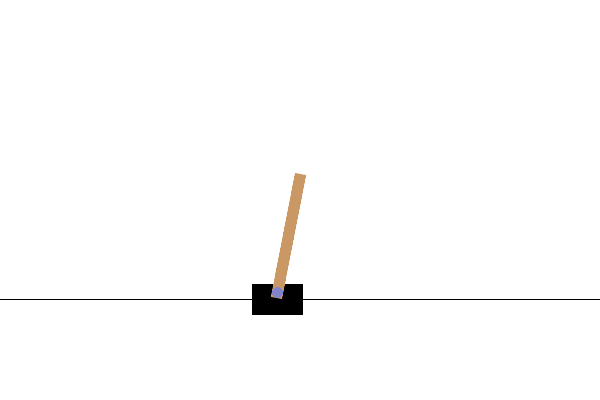
\includegraphics[width=0.5\textwidth]{Figures/cart_pole.png}
	\caption{The CartPole environment.}
\end{figure}
The CartPole environment is the "Hello World" of reinforcement learning; it describes a game where at each timestep, the aim is to balance a mass above a slider, 1 point is given for each timestep that the mass makes an angle of fewer than 12 degrees from vertical, in this instantiation. The action space$a \in {0,1}$, for the problem, is to either push the pole left or right. The state space is the position of the cart, the velocity of the cart, the angle of the pole and the angular velocity of the pole. A state is a vector s:
\begin{equation}
	s = \begin{pmatrix}
		x       \\
		\dot{x} \\
		\theta  \\
		\dot{\theta}
	\end{pmatrix}
\end{equation}
Thus, $s \in \mathbb{R}^4$.

Typically, the episodes are truncated at 500 timesteps, and the reward is 1, so the return is an integer $G_0 \in [0, 500]$. An episode terminates if the pole falls over or the cart moves too far from the centre. If a human were learning to solve this problem, one would notice that the expected result of pushing the cart left when it is leaning right at some positions is the same as pushing the cart right when it is leaning left at the displacement in the opposite direction. This is an example of symmetry in the problem, and it is this symmetry that is exploited by~\cite{vanderpol2020mdp, mondal2020group}.

To learn the transition dynamics of CartPole and agent must learn how the system evolves through time. In CartPole the transitions between different states in CartPole are governed by the PDEs:

\begin{equation}
	\ddot{\theta} = \frac{g \sin \theta + \cos\theta \left({\frac{-F - m_p l \dot{\theta}^2 \sin(\theta)}{m_c + m_p}} \right )}{l\left ( \frac{4}{3} - \frac{m_p \cos^2 \theta}{m_c + m_p}\right)},
\end{equation}

\begin{equation}
	\ddot{x} = \frac{ F + m_p l (\dot{\theta}^2 \sin \theta - \ddot{\theta} \cos \theta)}{m_c + m_p}.
\end{equation}
Here $g$ is the acceleration due to gravity and is positive, $\theta$ is the angle between the pole and vertical, with the pole length $l$. $F$ is the action force, where the positive direction is right. The masses of the cart and the pole are $m_c, m_p$, respectively. Finally $\dot{}$, indicates a derivative with respect to time.

These PDEs have no closed solution and their form is taken from \cite{florian2007correct} who provides slight corrections to the original dynamics in \cite{barto1983neuronlike}.

Both learning a policy and a transition model may be augmented by exploiting symmetry. The symmetry present in CartPole is the cyclic $C_2$ group. Other than the trivial group, the group with a single element, the $C_2$ group, is the simplest. This is a group with only two elements, the identity and inversion.
\begin{table}[h!]\label{tab:c2}
	\centering
	\begin{tabular}{c | c  c}
		$C_2$ & $e$ & $r$ \\
		\hline
		$e$   & $e$ & $r$ \\
		$r$   & $r$ & $e$
	\end{tabular}
	\caption{The $C_2$ group table, where entry $i, j$ is the result of group operation on the $i^{th}$ and $j^{th}$ element.}
\end{table}


%%As such, to find the group structured MDP homomorphism, the agent needs to learn an equivariant mapping that respects $\pi_1^s\mathbf{s} = \mathbf{s}$ and $\pi_r^s\mathbf{s} = -\mathbf{s}$, as well as $\pi_1^a\mathbf{a} = \mathbf{a}$ and $\pi_r^a\mathbf{a} = 1 - \mathbf{a}$. Here the state and actions as vectors; $\mathbf{s}, \mathbf{a}$ are being acted upon by the vector representations of $C_2, \pi$ in their respective spaces.

\section{Catch}\label{sec:catch}
\begin{figure}
	\label{fig:catch_env}
	\centering
	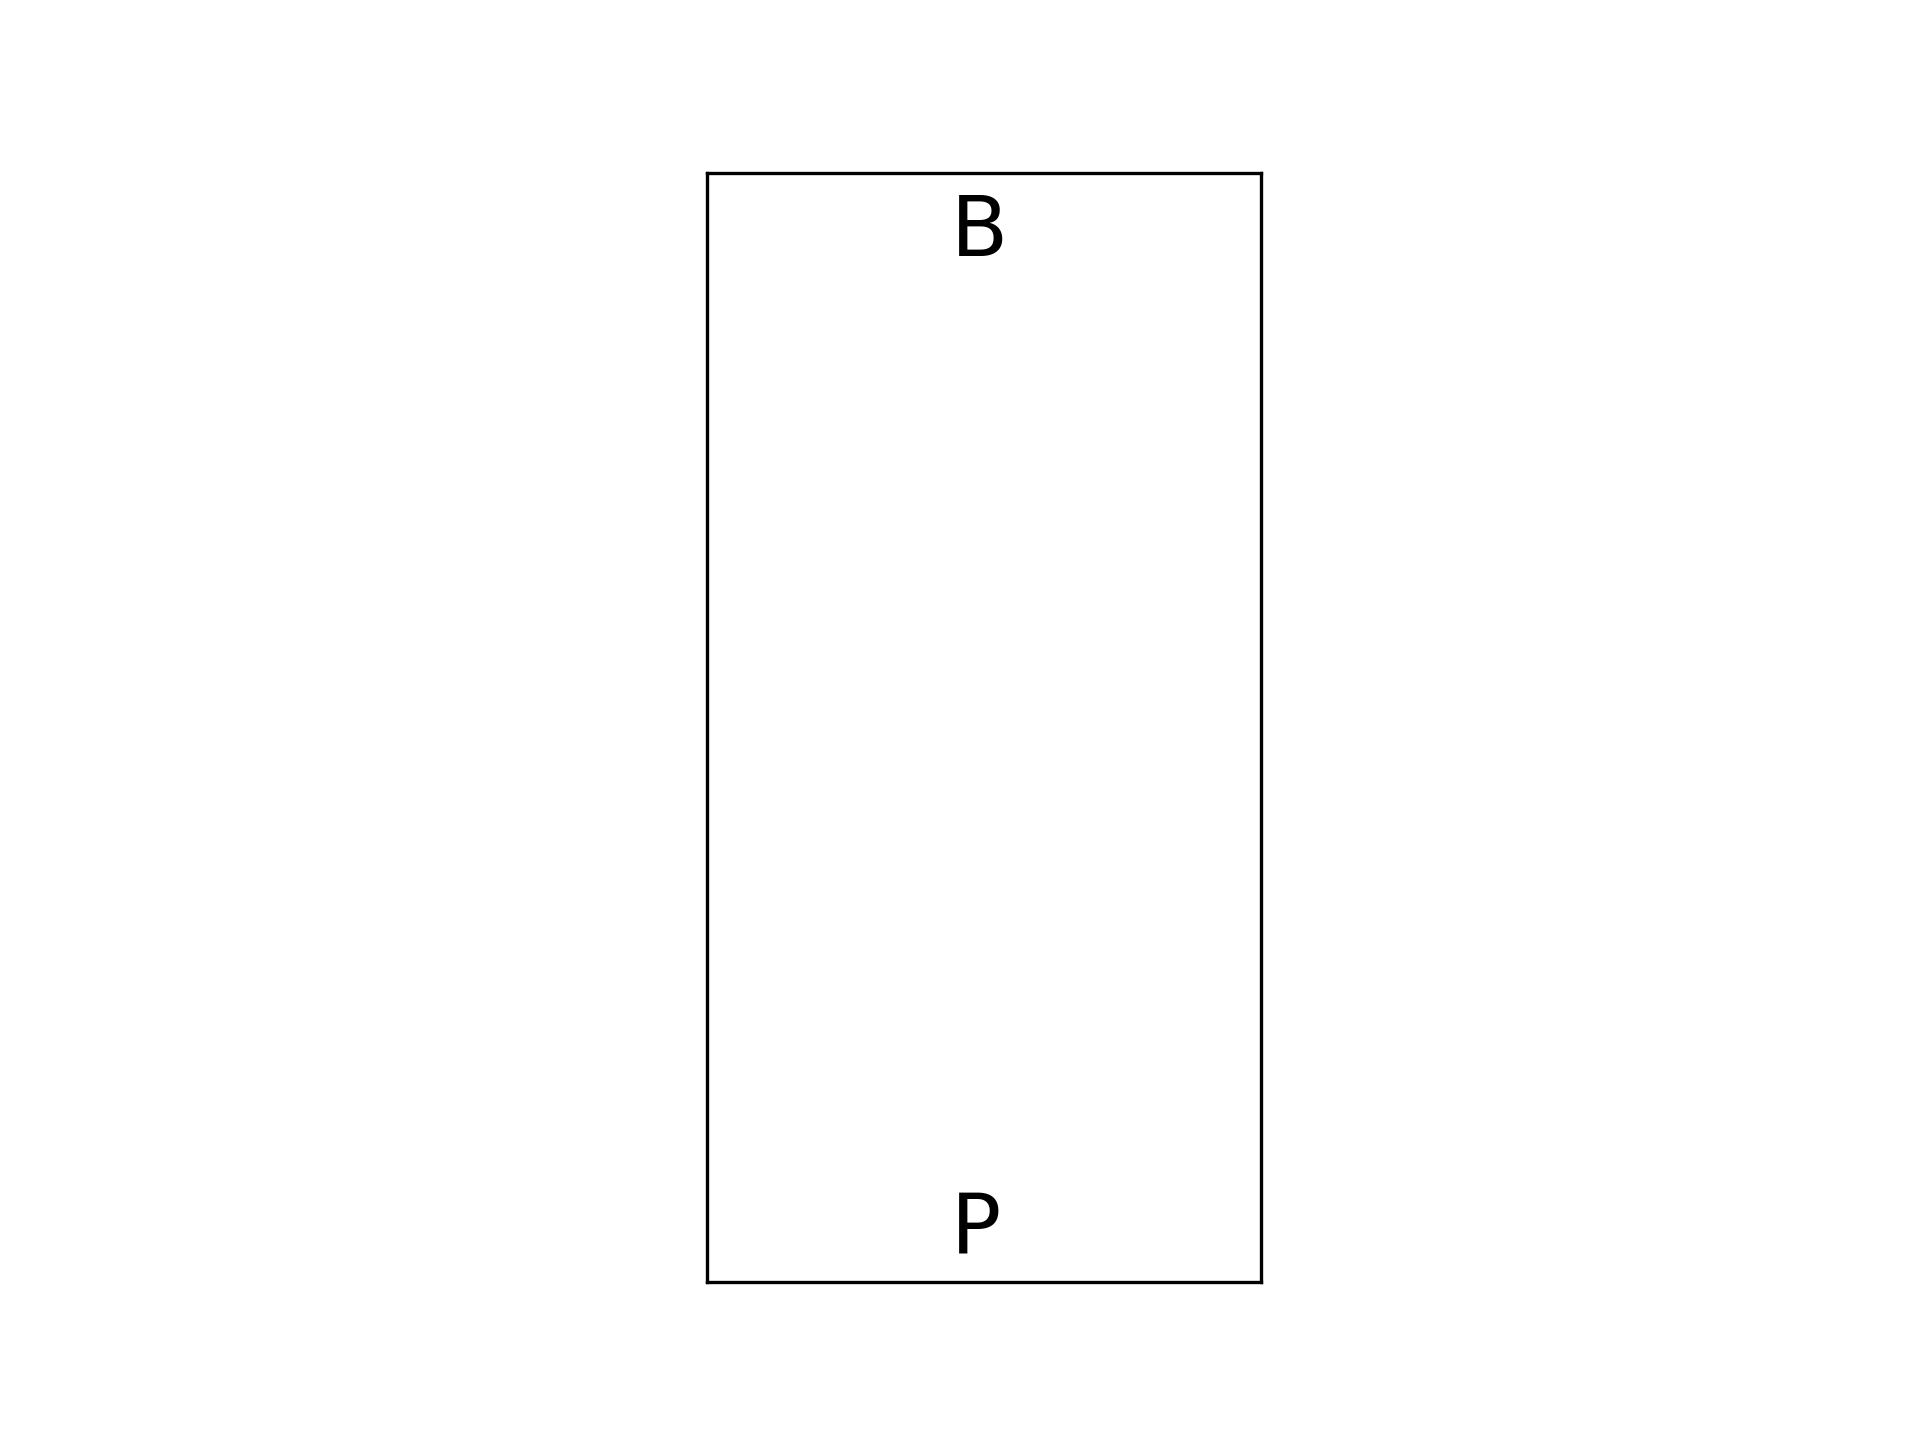
\includegraphics[width = 0.6\textwidth]{Figures/catch_env.png}
	\caption{The Catch environment. The ball position is indicated by B, and the paddle position is indicated by P.}
\end{figure}
The Catch environment~\cite{osband2020bsuite} is another simple MDP task similar to CartPole used mainly for debugging implementations. The aim of the game is to catch a falling ball. The default implementation has ten rows and 5 columns. The ball moves down by one row every time-step, and the position of the paddle is translated left or right by the action of the agent. When the ball reaches the tenth row, the reward of the system is $+1$, if the ball and the paddle are in the same location, otherwise the reward is $-1$. For all other time-steps the reward is 0. This produces an episodic environment, with a maximum return of $1$.

The state and action spaces are both discrete, and the transitions are deterministic. These states are represented to the agent as a $5\times 10$ array, with the ball and paddle's positions indicated by ones. The actions the agent can take are $\mathcal{A} = [0, 1, 2]$, that translate the ball by $1-a$. Thus, the MDP has a finite amount of transitions and state action pairs, 675.

Like CartPole, the Catch environment possesses $C_2$ group symmetry, however, due to the different state and action spaces the representations of the groups are different. However, because the groups are the same the structure is that in Table~\ref{tab:c2}.



\section{Neural Networks and Inductive Biases}

What is nice in many ways about the original MLP model is that it is so flexible. An infinite width MLP may produce any function~\cite{hornik1989multilayer}. However, this also highlights one of their weaknesses when solving applied problems, because in theory MLPs have incredible expressive power, they are perfectly able to represent physically impossible functions. When applied to domains such as images, and physical processes where there are concrete rules governing the processes that are being modelled. Additionally, it is posited by~\cite{wolpert1995no}, that there is no free lunch in machine learning, and that there must be a constrained search space for possible algorithms. Such constraints are in other words, inductive biases~\cite{baxter2000model}. This kind of reasoning has lead to research into encoding inductive biases into Deep Networks, from~\cite{goyal2022inductive} a table of current approaches to introduce inductive biases;

\begin{table}
	\centering
	\begin{tabular}{|c | c|}
		\hline
		Inductive Bias              & Corresponding property                              \\
		\hline
		\hline
		Distributed representations & Inputs mapped to patterns of features               \\
		\hline
		Convolution                 & group equivariance (usually over space)             \\
		\hline
		Deep architectures          & Complicated functions = composition of simpler ones \\
		\hline
		Graph Neural Networks       & equivariance over entities and relations            \\
		\hline
		Recurrent Nets              & equivariance over time                              \\
		\hline
		Soft attention              & equivariance over permutations                      \\
		\hline
		Self-supervised             & pre-training $P(X)$ is informative about $P(Y |X)$  \\
		\hline
	\end{tabular}
\end{table}

For the purposes of this thesis, the focus will be on the induction of group equivariances. However, it is important to note that this strategy to improving machine learning models comes from a more general class of ideas.


\subsection{G-CNNs}\label{sec:G-CNNs}

The Group Equivariant Convolutional Neural Network (G-CNN) is a generalization of the CNN's translational equivariance to arbitrary group structured equivariances.

The traditional Convolution layer is a discrete convolution, this is an approximation of the continuous convolution,
\begin{equation}
	(f*k)(x) = \int_{\mathbb{R}^d} k(x-x')f(x')dy,
\end{equation}
where $f$ and $k$ are functions on $\mathbb{R}^d$. What can be noticed is that this is the definition of the cross correlation between $f$ and $\ell_g[k]:  \mathbb{R}^d  \rightarrow \mathbb{R}^d$, where $\ell_g[k]$
is the translation group $\mathbb{R}^d$ acting on the kernel $k$,
\begin{align}
	(f*k)(x) & = \int_{\mathbb{R}^d} k(x-x')f(x')dx'       \\
	         & = \int_{\mathbb{R}^d} k(g^{-1}x')f(x')dx'   \\
	         & = \int_{\mathbb{R}^d} \ell_g[k](x')f(x')dx'
\end{align}
Here, the inverse of a translation by $x$, group action $g$ is the translation by $-x$. This is then $g^{-1}$, the inverse of the group action. To demonstrate the equivariance, consider a group action on the function $f$;
\begin{align}
	(\ell_g[f]* k) & = \int_{\mathbb{R}^d} \ell_g[k](x')\ell_g[f](x')dx' \\
	               & = \ell_g[\int_{\mathbb{R}^d} k(x')f(x')dx']         \\
	               & = \ell_g[(f * k)]
\end{align}
Thus, the layers are equivariant. When implementing this in practice, it amounts to applying all transformations to a single kernel that defines the trainable parameters for a layer. This is discussed in more detail in~\ref{sec:Actor-Critic}.

This is the backbone of the G-CNN\cite{cohen2016group}, where rather than a translation group, we have an arbitrary group $G$ acting on the kernel $k$. When looking for more complex equivariances than $C_2$, multiple different groups can be used in the same layer, this increases the number of variables in the convolution's output, this complicates the form of the layers, however for our purposes this is not relevant.



